\uuid{djCi}
\titre{Classification des points d'un triangle}
\theme{réseaux de neurones}
\auteur{Maxime NGUYEN}
\organisation{AMSCC}
\datecreate{13/12/2024}
\contenu{
	
\texte{ 	On souhaite construire un réseau de neurones qui réalise une classification des points du plan $\R^2$ selon que ces points appartiennent ou non au triangle $T$ dont les sommets sont les points de coordonées respectives $(-1,-1),(-1,1),(1,1)$ comme ci-dessous.
	
	\begin{center}
		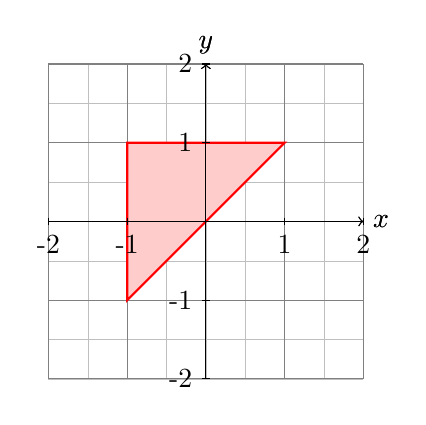
\begin{tikzpicture}[scale=1]
			
			% Grille avec un pas de 0.2 en gris clair
			\draw[step=0.5,lightgray,very thin] (-2,-2) grid (2,2);
			\draw[step=1,gray, thin] (-2,-2) grid (2,2);
			% Axes
			\draw[->] (-2,0) -- (2,0) node[right] {$x$};
			\draw[->] (0,-2) -- (0,2) node[above] {$y$};
			% Dessin du triangle
			\filldraw[thick,red,fill=red!20] (-1,-1) -- (-1,1) -- (1,1) -- cycle;
			% Axes
			\draw[->] (-2,0) -- (2,0) node[right] {$x$};
			\draw[->] (0,-2) -- (0,2) node[above] {$y$};
			
			% Ticks sur l'axe x
			\foreach \x in {-2,-1,1,2} {
				\draw (\x,0.05) -- (\x,-0.05) node[below] {\x};
			}
			% Ticks sur l'axe y
			\foreach \y in {-2,-1,1,2} {
				\draw (0.05,\y) -- (-0.05,\y) node[left] {\y};
			}
			
			
			
			
		\end{tikzpicture}
	\end{center} }
	
	\begin{enumerate}
		\item \question{ Démontrer que le perceptron défini ci-dessous réalise l'opération logique $x$ ET $y$ ET $z$ où $(x,y,z) \in \{0,1\}^3$. 
		
		\begin{center}
			\begin{tikzpicture}[scale=0.3, font=\scriptsize]
				
				\draw[thick,fill=black!10] (0,0) circle (3);
				\draw[ultra thick]  (150:3) -- (150:8)node[pos=0.2,above]{$1$} node[left]{$x$};
				\draw[ultra thick]  (170:3) -- (170:8)node[pos=0.2,above]{$1$} node[left]{$y$};
				\draw[ultra thick]  (190:3) -- (190:8)node[pos=0.2,above]{$1$} node[left]{$z$};
				\draw[-o,ultra thick]  (210:3) -- (210:8) node[pos=0.2,below]{$-3$};
				\draw[->,>=latex,ultra thick] (0:3) --  (8,0);
				\node[below right] at (-15:3) {$H$};
				
			\end{tikzpicture}  }
		\end{center} 
		\item \question{ En déduire un réseau de neurones prenant un vecteur $(x,y) \in \R^2$ en entrée et renvoyant 
		$1$ si $(x,y) \in T$, $0$ sinon.  }
		\item \question{ Soit $P$ un polygône convexe du plan à 10 côtés. Décrire l'architecture d'un réseau de neurones permettant de réaliser une classification des points appartenant à l'intérieur de ce polygône.  }
	\end{enumerate}
	
}